%%%%%%%%%%%%%%%%%%%%%%%%%%%%%%%%%%%%%%%%%
% Beamer Presentation
% LaTeX Template
% Version 1.0 (10/11/12)
%
% This template has been downloaded from:
% http://www.LaTeXTemplates.com
%
% License:
% CC BY-NC-SA 3.0 (http://creativecommons.org/licenses/by-nc-sa/3.0/)
%
%%%%%%%%%%%%%%%%%%%%%%%%%%%%%%%%%%%%%%%%%

%----------------------------------------------------------------------------------------
%	PACKAGES AND THEMES
%----------------------------------------------------------------------------------------

\documentclass{beamer}

\mode<presentation> {

% The Beamer class comes with a number of default slide themes
% which change the colors and layouts of slides. Below this is a list
% of all the themes, uncomment each in turn to see what they look like.

%\usetheme{default}
%\usetheme{AnnArbor}
%\usetheme{Antibes}
%\usetheme{Bergen}
%\usetheme{Berkeley}
%\usetheme{Berlin}
%\usetheme{Boadilla}
%\usetheme{CambridgeUS}
%\usetheme{Copenhagen}
%\usetheme{Darmstadt}
%\usetheme{Dresden}
%\usetheme{Frankfurt}
%\usetheme{Goettingen}
%\usetheme{Hannover}
%\usetheme{Ilmenau}
%\usetheme{JuanLesPins}
%\usetheme{Luebeck}
\usetheme{Madrid}
%\usetheme{Malmoe}
%\usetheme{Marburg}
%\usetheme{Montpellier}
%\usetheme{PaloAlto}
%\usetheme{Pittsburgh}
%\usetheme{Rochester}
%\usetheme{Singapore}
%\usetheme{Szeged}
%\usetheme{Warsaw}

% As well as themes, the Beamer class has a number of color themes
% for any slide theme. Uncomment each of these in turn to see how it
% changes the colors of your current slide theme.

%\usecolortheme{albatross}
%\usecolortheme{beaver}
%\usecolortheme{beetle}
%\usecolortheme{crane}
%\usecolortheme{dolphin}
%\usecolortheme{dove}
%\usecolortheme{fly}
%\usecolortheme{lily}
%\usecolortheme{orchid}
%\usecolortheme{rose}
%\usecolortheme{seagull}
%\usecolortheme{seahorse}
%\usecolortheme{whale}
%\usecolortheme{wolverine}

%\setbeamertemplate{footline} % To remove the footer line in all slides uncomment this line
%\setbeamertemplate{footline}[page number] % To replace the footer line in all slides with a simple slide count uncomment this line

%\setbeamertemplate{navigation symbols}{} % To remove the navigation symbols from the bottom of all slides uncomment this line
}
\usepackage{ngerman}
\usepackage[utf8]{inputenc}
\usepackage[T1]{fontenc}	
\usepackage{textcomp}
\usepackage{graphicx} % Allows including images
\usepackage{booktabs} % Allows the use of \toprule, \midrule and \bottomrule in tables
\usepackage{animate}

%----------------------------------------------------------------------------------------
%	TITLE PAGE
%----------------------------------------------------------------------------------------

\title[Cut \& Count]{Implementierung der Cut \& Count-Technik am Beispiel Steiner tree} % The short title appears at the bottom of every slide, the full title is only on the title page

\author{
Levin von Hollen, 
Tilman Beck
}
\institute[] % Your institution as it will appear on the bottom of every slide, may be shorthand to save space
{
\textit{ \{stu127560-, stu127568-\}@informatik.uni-kiel.de} \\
\medskip
Christian-Albrechts Universität Kiel  % Your institution for the title page
}
\date{\today} % Date, can be changed to a custom date

\begin{document}

\begin{frame}
\titlepage % Print the title page as the first slide
\end{frame}

\begin{frame}
\frametitle{Überblick} % Table of contents slide, comment this block out to remove it
\tableofcontents % Throughout your presentation, if you choose to use \section{} and \subsection{} commands, these will automatically be printed on this slide as an overview of your presentation
\end{frame}

%----------------------------------------------------------------------------------------
%	PRESENTATION SLIDES
%----------------------------------------------------------------------------------------

%------------------------------------------------
\section{Cut \& Count} % Sections can be created in order to organize your presentation into discrete blocks, all sections and subsections are automatically printed in the table of contents as an overview of the talk
%------------------------------------------------
\subsection{Allgemeines}
\begin{frame}
\frametitle{Cut \& Count-Technik}
\begin{itemize}
\item Technik um connectivity-type Probleme mithilfe von Randomisierung zu lösen(Marek Cygan, Jesper Nederlof, Marcin Pilipczuk, Michał Pilipczuk, Johan van Rooij, Jakub Onufry Wojtaszczyk)
\item angewendet auf viele verschiedene Probleme (z.B. Longest Path, Steiner Tree, Feedback Vertex Set, uvm.)
\item Randomisierung durch Isolation-Lemma 
\item als Ergebnis ein einseitiger Monte-Carlo-Algorithmus mit Laufzeit $c^{tw(G)} |V|^{\mathcal{O}(1)}$
%\note{kurz erklären: connectivity-type Probleme, Isolation Lemma, Laufzeit, einseitig, montecarlo }
\end{itemize}
\end{frame}

\begin{frame}
\frametitle{Cut \& Count-Technik}
\begin{block}{Theorem}
There exist Monte-Carlo algorithms that given a tree decomposition of the (underlying undirected
graph of the) input graph of width $t$ solve the following problems:
\begin{itemize}
\item Steiner Tree in $3^t|V|^{\mathcal{O}(1)}$
\item Feedback Vertex Set in $3^t|V|^{\mathcal{O}(1)}$
\item \dots
\end{itemize}
The algorithms cannot give false positives and may give false negatives with probability at most $1/2$.
\end{block}
\end{frame}

\section{Cut \& Count mit Steiner Tree} % A subsection can be created just before a set of slides with a common theme to further break down your presentation into chunks
\begin{frame}
\frametitle{Steiner Tree}
\begin{block}{Problem}
\textbf{Input}: An undirected graph $G = (V, E)$, a set of terminals $T \subseteq V$ and an integer $k$. \\
\textbf{Question}: Is there a set $X \subseteq V$ of cardinality $k$ such that $T \subseteq X$ and $G[X]$ is connected?
\end{block}
\end{frame}
\subsection{Cut}
\begin{frame}
\frametitle{Cut (1)}
\begin{itemize}
\item definiere Gewichtsfunktion $\omega:V\rightarrow \{1,\dots,N\}$ 
% alle Knoten erhalten ein zufälliges Gewicht -> später wichtig für Randomisierung, N = |V| für 1/2 Wahrscheinlichkeit
\item sei $\mathcal{R}_W$ die Menge aller Teilmengen von $X$ aus $V$ mit $T \subseteq X$, $\omega(X)=W$ und $|X|=k$
\item sei  $\mathcal{S}_W=\{X \in \mathcal{R}_W | G[X]$ ist zusammenhängend$\}$ 
\item $\cup_W \mathcal{S}_W$ ist die Menge der Lösungen
\item gibt es ein $W$ für das die Menge nichtleer ist, so gibt der Algorithmus eine positive Antwort
\end{itemize}
\end{frame}
%--------------------
\begin{frame}
\frametitle{Cut (2) - wozu $\omega$ ?}
\begin{itemize}
\item Gewichtsfunktion $\omega:V\rightarrow \{1,\dots,N\}$ 
\item der Algorithmus (ohne $\omega$) ist korrekt, sofern es \textbf{genau eine} oder \textbf{keine} Lösung gibt
\item mithilfe des Isolation Lemma kann mit hoher Wahrscheinlichkeit eine große Lösungsmenge auf eine einzige reduziert werden
\end{itemize}
\begin{block}{Isolation Lemma}
Let $\mathcal{F} \subseteq 2^U$ be a set family over a universe $U$ with $|\mathcal{F}| > 0$. For each $u \in U$ ,
choose a weight $\omega(u) \in {1, 2, . . . , N }$ uniformly and independently at random. Then
\begin{center}
$prob[\omega$ isolates $\mathcal{F}]\geq 1 - \frac{|U|}{N}$
\end{center}
\end{block}
\end{frame}
%--------------------
\begin{frame}
\frametitle{Cut (3)}
\begin{itemize}
\item einen beliebigen Terminalknoten $v \in T$ als $v_1$ festlegen
\item sei $\mathcal{C}_W$ die Menge aller Subgraphen, die einen konsistenten Cut $(X,(X_1,X_2))$ bilden, wobei $X\in \mathcal{R}_W$ und $v_1 \in X_1$ 
\newline
\newline
\begin{block}{Lemma 3.3}
Let $G=(V,E)$ be a graph and let $X$ be a subset of vertices such that $v_1 \in X \subseteq V$. The number of
consistently cut subgraphs $(X,(X_1,X_2))$ such that $v_1 \in X_1$ is equal to $2^{cc(G[X])-1}$.
\end{block}
%am Tafelbild erklären was ein consistent cut ist

\end{itemize}
\end{frame}

\subsection{Count}
\begin{frame}
\frametitle{Count (1)}
\begin{itemize}
\item aus Lemma 3.3 ist bekannt: $|\mathcal{C}|=\sum_{X \in \mathcal{R}} 2^{cc(G[X])-1}$
\item wir legen $W$ fest und ignorieren die Indices: $|\mathcal{C}| \equiv |\{X \in \mathcal{R} |cc(G[X]) = 1\}| = |\mathcal{S}|$
\end{itemize}
\begin{block}{Lemma 3.4}
Let $G,$ $\omega$, $\mathcal{C}_W$ and $\mathcal{S}_W$ be as defined above. Then for every $W$, $|\mathcal{S}_W| \equiv |\mathcal{C}_W|$.
\end{block}
\end{frame}
%-------------------------
\begin{frame}
\frametitle{Einschub: Tree Decomposition (1)}
\begin{block}{Tree Decomposition}
A tree decomposition of a graph $G$ is a tree $\mathbb{T}$ in which each vertex $x \in \mathbb{T}$ has an assigned set of vertices $B_x \subseteq V$ (called a bag) such that $\cup_{x \in \mathbb{T}} B_x = V$ with the following properties:
\begin{itemize}
\item for any $uv \in E$, there exists an $x \in \mathbb{T}$ such that $u,v \in B_x$
\item if $v \in B_x$ and $v \in B_y$, then $v \in B_z$ for all $z$ on the path from $x$ to $y$ in $\mathbb{T}$
\end{itemize}
\end{block}
Kann in polynomieller Zeit berechnet werden (Beweis: Ton Kloks. Treewidth, Computations and Approximations, volume 842 of Lecture Notes in Computer Science. Springer, 1994)
\end{frame}
%-------------------------
\begin{frame}
\frametitle{Einschub: Tree Decomposition (2)}
\begin{center}
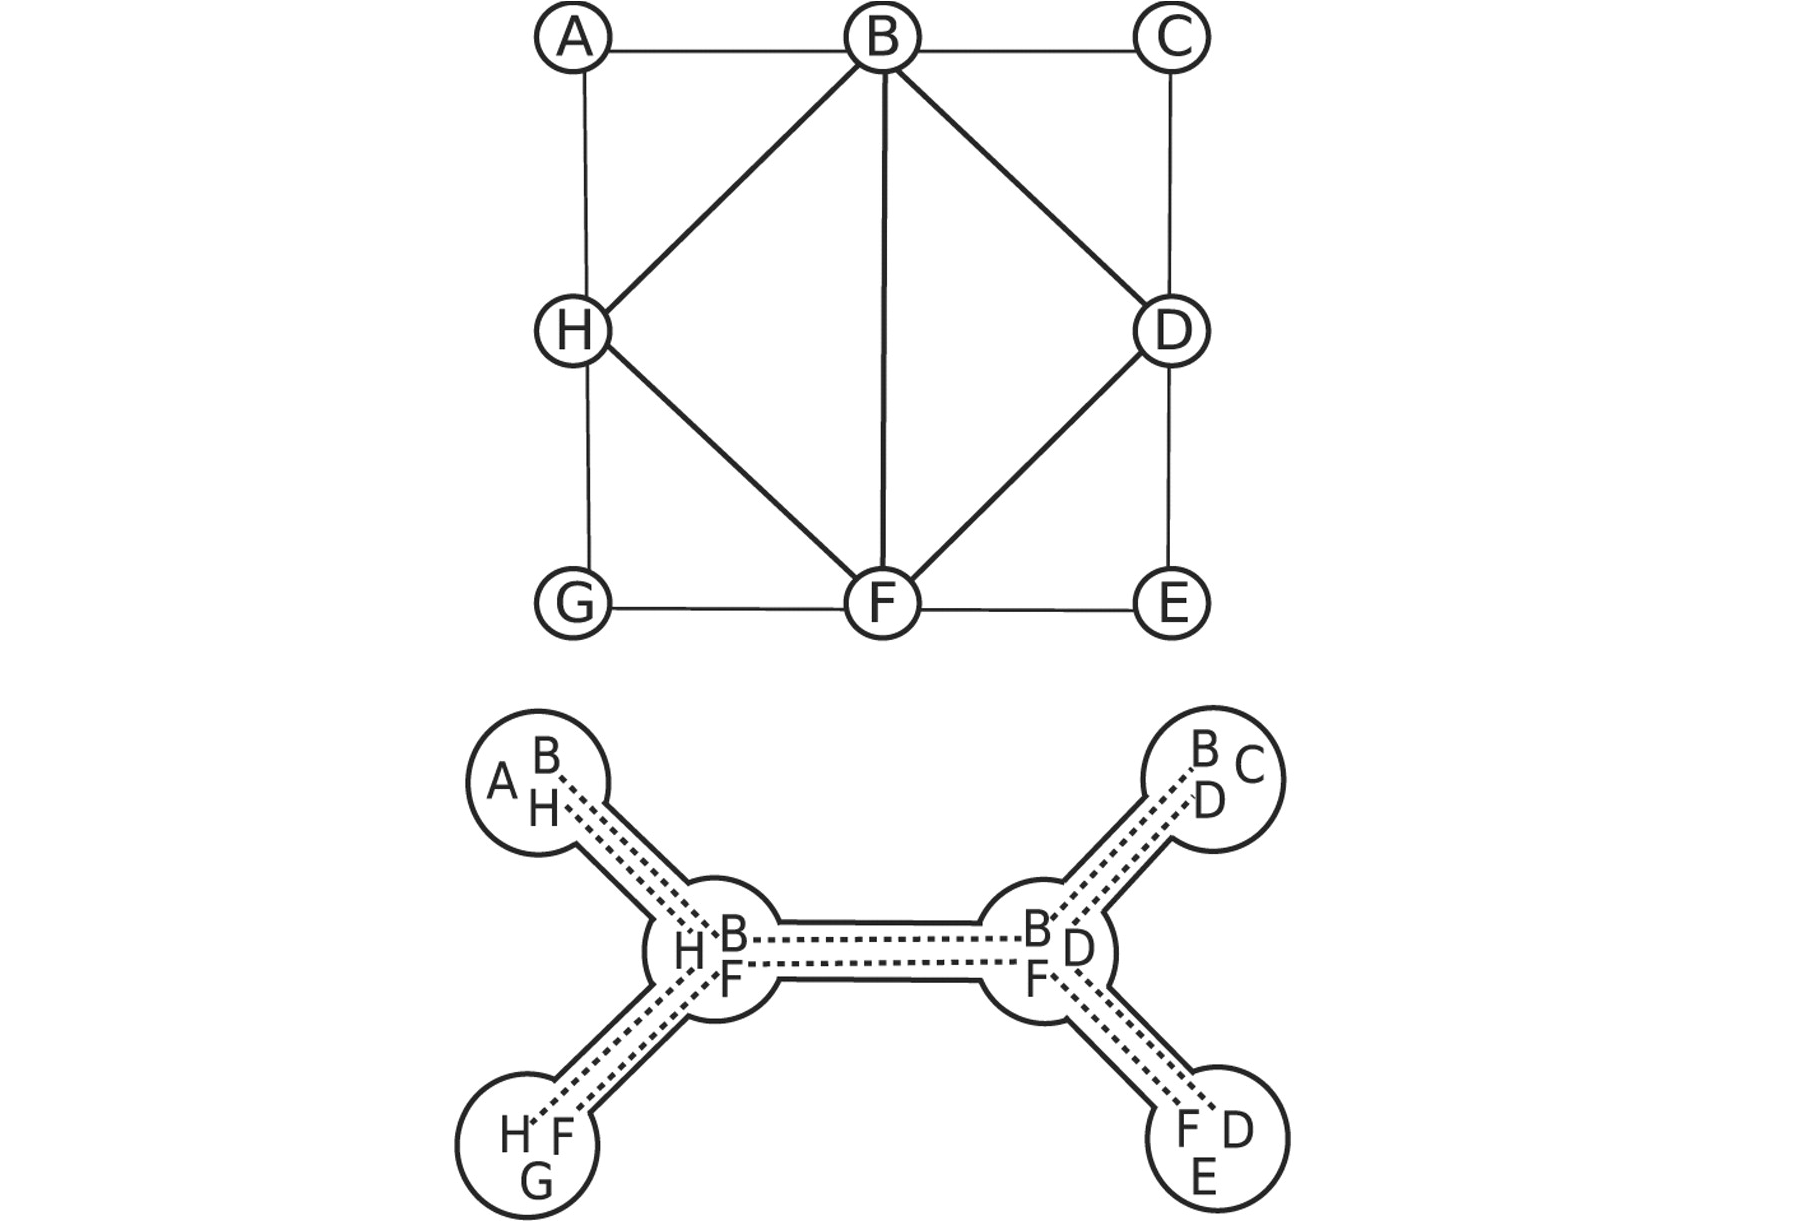
\includegraphics[scale=0.15]{./imgs/tree_decomposition1.png}
\end{center}
\end{frame}
%-------------------------
\begin{frame}
\frametitle{Einschub: Nice Tree Decomposition (NTD)}

\begin{center}
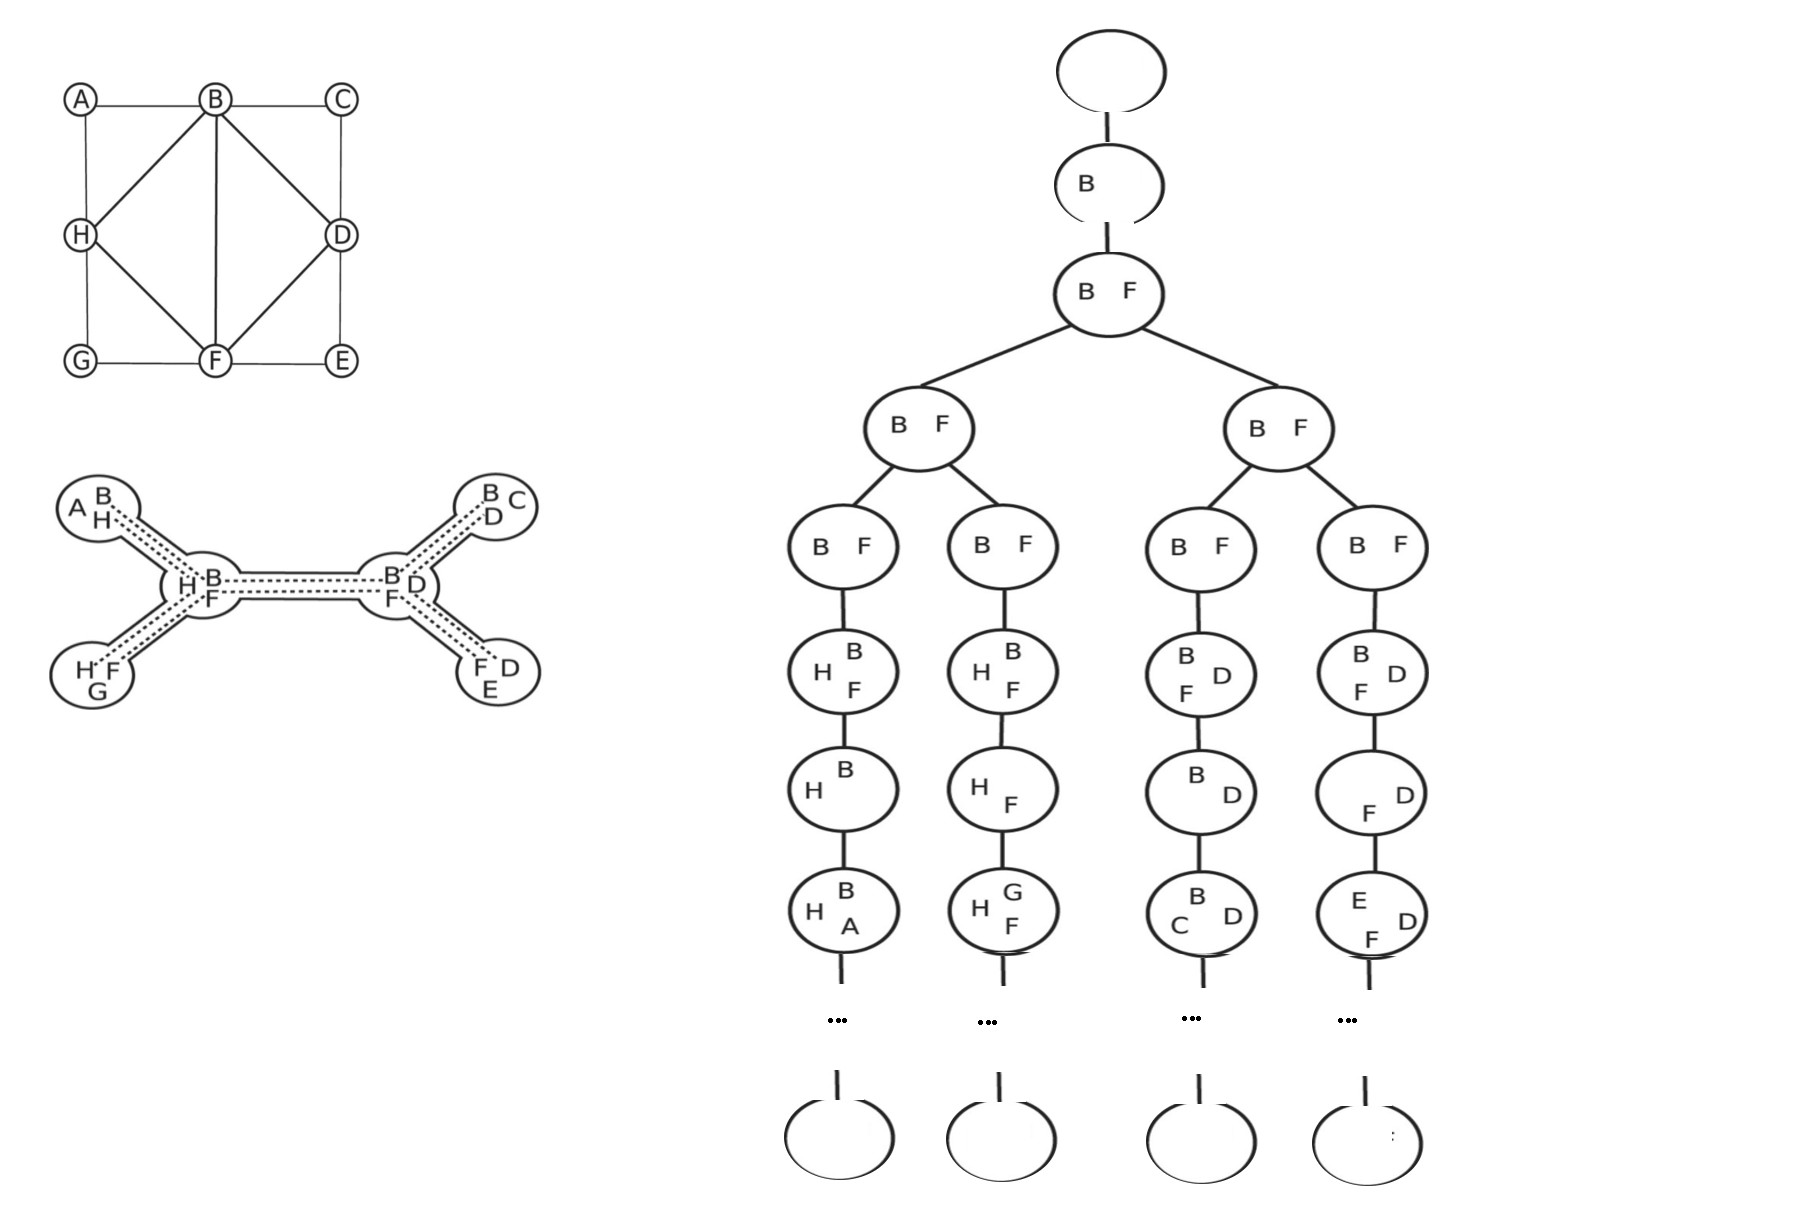
\includegraphics[scale=0.17]{./imgs/tree_decomposition2.jpg}
\end{center}
\note{jeder Knoten der NTD enthält einen Bag mit den Knoten aus dem Ursprungsgraphen und ein Label (leaf, root, introduce vertex, forget vertex, etc)}

%\item \textbf{Leaf bag}: a leaf $x$ of $\mathbb{T}$ with $B_x=\emptyset$
%\item \textbf{Introduce vertex bag}: an internal vertex $x$ of $\mathbb{T}$ with one child vertex $y$ for which $B_x = B_y %\cup \{v\}$ for some $v \notin B_y$. This bag is said to introduce $v$
%\item \textbf{Introduce edge bag}: an internal vertex $x$ of $\mathbb{T}$ labeled with an edge $uv \in E$ with one child %bag $y$ for which $u,v \in B_x = B_y$. This bag is said to introduce $uv$
%\item \textbf{Forget bag}: an internal vertex $x$ of $\mathbb{T}$ with one child bag $y$ for which $B_x=B_y \{v\}$ for %some $v \in B_y$. This bag is said to forget $v$
%\item \textbf{Join bag}: an internal vertex $x$ with two children vertices $l$ and $r$ with $B_r=B_l$
\end{frame}
%-------------------------
\begin{frame}
\frametitle{Count (2)}
\begin{itemize}
\item $|\mathcal{C}_W|$ modulo $2$ kann mit dynamischen Programm berechnet werden
\item für jeden Bag $x \in \mathbb{T}$, integers $0 \leq i \leq k,0 \leq w \leq kN$ und Färbung $s \in \{0,1_1,1_2 \}^{B_x}$ definiere:
\begin{itemize}
\item $\mathcal{R}_x(i,w)=\{X \subseteq V_x | (T \cap V_x) \subseteq X$ $\wedge$ $|X| = i$ $\wedge$ $\omega (X) = w \}$
\item $\mathcal{C} (i,w) =\{ (X,(X_1,X_2)) | X \in \mathcal{R}_x(i,w)$ $\wedge$ $(X,(X_1,X_2))$ is a consistently cut subgraph of $G_x$ $\wedge$ $(v_1 \in V_x \Rightarrow v_1 \in X_1 \} $
\item $\mathcal{A}_x(i,w,s)=| \{ (X,(X_1,X_2)) \in \mathcal{C}_x(i,w) | (s(v) = 1_j \Rightarrow v \in X_j)$ $\wedge$ $(s(v)=0 \Rightarrow v \notin X \} |$
\note{$\mathcal{R}_(i,w)$ enthält alle Mengen $X \subseteq V_x$, welche potenziell zu einer Lösung aus $\mathcal{R}$ erweitert werden können (mit Restriktion i und w), entsprechend enthält $\mathcal{C}_x(i,w)$ alle consistently cut Subgraphen}

\end{itemize}
\end{itemize}
\end{frame}
%-------------------------
\begin{frame}
\frametitle{Count (3)}
Färbung $s \in \{0,1_1,1_2 \}^{B_x}$
\begin{itemize}
\item $s[v] = 0 \Rightarrow v \notin X$
\item $s[v] = 1_1 \Rightarrow v \in X_1$ 
\item $s[v] = 1_2 \Rightarrow v \in X_2$ 
\item $\mathcal{A}_x(i,w,s)$ zählt die Elemente $\mathcal{C}_x(i,w)$, die entsprechend gefärbt sind
\item $\sum\limits_{s \in  \{ 0,1_1,1_2 \}^{B_x} } A_x(i,w,s) = |C_x(i,w)|$
\item für die Lösung nur $A_r(k,W,\emptyset) = |C_r(k,W)| = |C_W|$ interessant (für alle W)
\item ausgehend von Wurzel-Knoten rekursiver Abstieg zu den Blatt-Knoten der NTD
\end{itemize}
\end{frame}
%-------------------------
\begin{frame}
\frametitle{Count (3)}
\begin{theorem}[Lemma 3.5]
Given $G=(V,E), T \subseteq V,$ an integer $k, \omega:V\rightarrow \{1,\dots,N \}$ and a nice tree decomposition $\mathbb{T}$, there exists an algorithm that can determine $|\mathcal{C}_W|$ modulo 2 for every $0 \leq W \leq kN$ in $3^tN^2|V|^{\mathcal{O}(1)}$ (t is the treewidth of the NTD)
\end{theorem}
\end{frame}

%------------------------------------------------
\section{Implementierung}
\begin{frame}
\frametitle{Implementierung}
\begin{columns}[c] % The "c" option specifies centered vertical alignment while the "t" option is used for top vertical alignment

\column{.45\textwidth} % Left column and width
\begin{itemize}
\item Inorder-Traversierung der NTD
\item Berechnung einer Datenmatrix basierend auf dynamischen Programm und Kind-Knoten
\item Wurzel- und alle Blattknoten enthalten 2D Datenmatrix
\end{itemize}

\column{.5\textwidth} % Right column and width
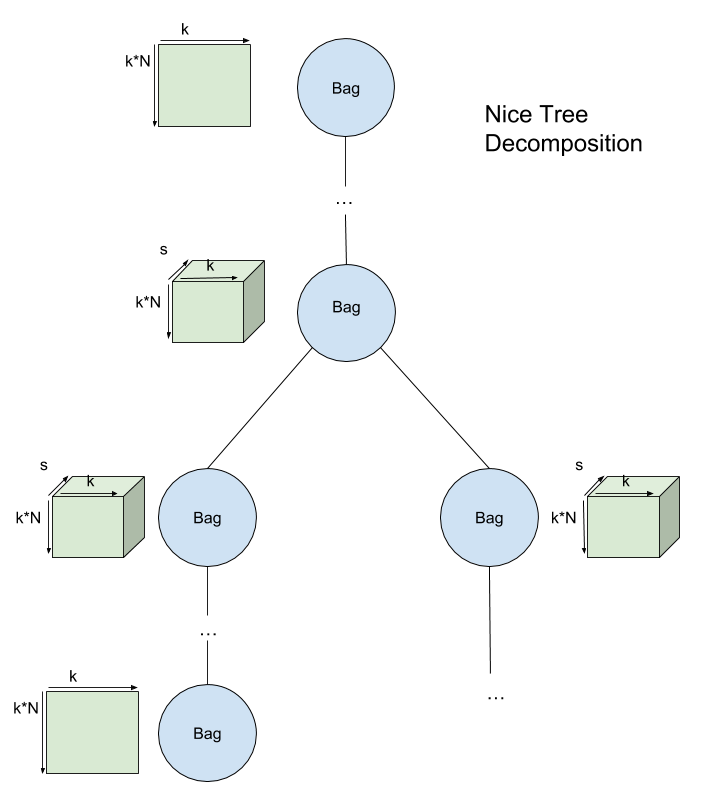
\includegraphics[scale=0.25]{./imgs/implementation.png}

\end{columns}
\end{frame}

%------------------------------------------------

\begin{frame}
\frametitle{dynamisches Programm}
\begin{block}{Berechnungen}
sei v der \glqq \textit{introduced vertex}\grqq in einem Introduced Vertex, sei y bzw. z der linke bzw. rechte Kind-Knoten von Bag x in der NTD, falls vorhanden
\begin{itemize}
\item \textbf{Leaf bag}:
\begin{itemize}
\item $A_x=(0,0,\emptyset) = 1$
\end{itemize}
\item \textbf{Introduce vertex v}:
\begin{itemize}
\item $A_x=(i,w,s[v\rightarrow 0]) = 1[v \notin T]A_y(i,w,s)$
\item test
\end{itemize}
\end{itemize}
\end{block}
\end{frame}

%------------------------------------------------

\begin{frame}
\frametitle{Multiple Columns}
\begin{columns}[c] % The "c" option specifies centered vertical alignment while the "t" option is used for top vertical alignment

\column{.45\textwidth} % Left column and width
\textbf{Heading}
\begin{enumerate}
\item Statement
\item Explanation
\item Example
\end{enumerate}

\column{.5\textwidth} % Right column and width
Lorem ipsum dolor sit amet, consectetur adipiscing elit. Integer lectus nisl, ultricies in feugiat rutrum, porttitor sit amet augue. Aliquam ut tortor mauris. Sed volutpat ante purus, quis accumsan dolor.

\end{columns}
\end{frame}

%------------------------------------------------

\begin{frame}
\frametitle{Table}
\begin{table}
\begin{tabular}{l l l}
\toprule
\textbf{Treatments} & \textbf{Response 1} & \textbf{Response 2}\\
\midrule
Treatment 1 & 0.0003262 & 0.562 \\
Treatment 2 & 0.0015681 & 0.910 \\
Treatment 3 & 0.0009271 & 0.296 \\
\bottomrule
\end{tabular}
\caption{Table caption}
\end{table}
\end{frame}

%------------------------------------------------

\begin{frame}
\frametitle{Theorem}
\begin{theorem}[Mass--energy equivalence]
$E = mc^2$
\end{theorem}
\end{frame}

%------------------------------------------------

\begin{frame}[fragile] % Need to use the fragile option when verbatim is used in the slide
\frametitle{Verbatim}
\begin{example}[Theorem Slide Code]
\begin{verbatim}
\begin{frame}
\frametitle{Theorem}
\begin{theorem}[Mass--energy equivalence]
$E = mc^2$
\end{theorem}
\end{frame}\end{verbatim}
\end{example}
\end{frame}

%------------------------------------------------

\begin{frame}
\frametitle{Figure}
Uncomment the code on this slide to include your own image from the same directory as the template .TeX file.
%\begin{figure}
%\includegraphics[width=0.8\linewidth]{test}
%\end{figure}
\end{frame}

%------------------------------------------------

\begin{frame}[fragile] % Need to use the fragile option when verbatim is used in the slide
\frametitle{Citation}
An example of the \verb|\cite| command to cite within the presentation:\\~

This statement requires citation \cite{p1}.
\end{frame}

%------------------------------------------------

\begin{frame}
\frametitle{References}
\footnotesize{
\begin{thebibliography}{99} % Beamer does not support BibTeX so references must be inserted manually as below
\bibitem[Smith, 2012]{p1} John Smith (2012)
\newblock Title of the publication
\newblock \emph{Journal Name} 12(3), 45 -- 678.
\end{thebibliography}
}
\end{frame}

%------------------------------------------------

\begin{frame}
\Huge{\centerline{Fragen?}}
\end{frame}

%----------------------------------------------------------------------------------------

\end{document} 